\documentclass[twoside]{book}

% Packages required by doxygen
\usepackage{fixltx2e}
\usepackage{calc}
\usepackage{doxygen}
\usepackage[export]{adjustbox} % also loads graphicx
\usepackage{graphicx}
\usepackage[utf8]{inputenc}
\usepackage{makeidx}
\usepackage{multicol}
\usepackage{multirow}
\PassOptionsToPackage{warn}{textcomp}
\usepackage{textcomp}
\usepackage[nointegrals]{wasysym}
\usepackage[table]{xcolor}

% Font selection
\usepackage[T1]{fontenc}
\usepackage[scaled=.90]{helvet}
\usepackage{courier}
\usepackage{amssymb}
\usepackage{sectsty}
\renewcommand{\familydefault}{\sfdefault}
\allsectionsfont{%
  \fontseries{bc}\selectfont%
  \color{darkgray}%
}
\renewcommand{\DoxyLabelFont}{%
  \fontseries{bc}\selectfont%
  \color{darkgray}%
}
\newcommand{\+}{\discretionary{\mbox{\scriptsize$\hookleftarrow$}}{}{}}

% Page & text layout
\usepackage{geometry}
\geometry{%
  a4paper,%
  top=2.5cm,%
  bottom=2.5cm,%
  left=2.5cm,%
  right=2.5cm%
}
\tolerance=750
\hfuzz=15pt
\hbadness=750
\setlength{\emergencystretch}{15pt}
\setlength{\parindent}{0cm}
\setlength{\parskip}{3ex plus 2ex minus 2ex}
\makeatletter
\renewcommand{\paragraph}{%
  \@startsection{paragraph}{4}{0ex}{-1.0ex}{1.0ex}{%
    \normalfont\normalsize\bfseries\SS@parafont%
  }%
}
\renewcommand{\subparagraph}{%
  \@startsection{subparagraph}{5}{0ex}{-1.0ex}{1.0ex}{%
    \normalfont\normalsize\bfseries\SS@subparafont%
  }%
}
\makeatother

% Headers & footers
\usepackage{fancyhdr}
\pagestyle{fancyplain}
\fancyhead[LE]{\fancyplain{}{\bfseries\thepage}}
\fancyhead[CE]{\fancyplain{}{}}
\fancyhead[RE]{\fancyplain{}{\bfseries\leftmark}}
\fancyhead[LO]{\fancyplain{}{\bfseries\rightmark}}
\fancyhead[CO]{\fancyplain{}{}}
\fancyhead[RO]{\fancyplain{}{\bfseries\thepage}}
\fancyfoot[LE]{\fancyplain{}{}}
\fancyfoot[CE]{\fancyplain{}{}}
\fancyfoot[RE]{\fancyplain{}{\bfseries\scriptsize Generated by Doxygen }}
\fancyfoot[LO]{\fancyplain{}{\bfseries\scriptsize Generated by Doxygen }}
\fancyfoot[CO]{\fancyplain{}{}}
\fancyfoot[RO]{\fancyplain{}{}}
\renewcommand{\footrulewidth}{0.4pt}
\renewcommand{\chaptermark}[1]{%
  \markboth{#1}{}%
}
\renewcommand{\sectionmark}[1]{%
  \markright{\thesection\ #1}%
}

% Indices & bibliography
\usepackage{natbib}
\usepackage[titles]{tocloft}
\setcounter{tocdepth}{3}
\setcounter{secnumdepth}{5}
\makeindex

% Hyperlinks (required, but should be loaded last)
\usepackage{ifpdf}
\ifpdf
  \usepackage[pdftex,pagebackref=true]{hyperref}
\else
  \usepackage[ps2pdf,pagebackref=true]{hyperref}
\fi
\hypersetup{%
  colorlinks=true,%
  linkcolor=blue,%
  citecolor=blue,%
  unicode%
}

% Custom commands
\newcommand{\clearemptydoublepage}{%
  \newpage{\pagestyle{empty}\cleardoublepage}%
}

\usepackage{caption}
\captionsetup{labelsep=space,justification=centering,font={bf},singlelinecheck=off,skip=4pt,position=top}

%===== C O N T E N T S =====

\begin{document}

% Titlepage & ToC
\hypersetup{pageanchor=false,
             bookmarksnumbered=true,
             pdfencoding=unicode
            }
\pagenumbering{alph}
\begin{titlepage}
\vspace*{7cm}
\begin{center}%
{\Large Basic robot project }\\
\vspace*{1cm}
{\large Generated by Doxygen 1.8.13}\\
\end{center}
\end{titlepage}
\clearemptydoublepage
\pagenumbering{roman}
\tableofcontents
\clearemptydoublepage
\pagenumbering{arabic}
\hypersetup{pageanchor=true}

%--- Begin generated contents ---
\chapter{Main Page}
\label{index}\hypertarget{index}{}\hypertarget{index_Outline}{}\section{Outline}\label{index_Outline}
This project is created to learn following concepts
\begin{DoxyEnumerate}
\item Robot kinematics~\newline

\item Planning and navigation~\newline

\item Datastructures and algorithms~\newline

\item C++ \& R\+OS~\newline

\item Production grade software development 
\end{DoxyEnumerate}
\chapter{Hierarchical Index}
\section{Class Hierarchy}
This inheritance list is sorted roughly, but not completely, alphabetically\+:\begin{DoxyCompactList}
\item Controller\begin{DoxyCompactList}
\item \contentsline{section}{rear\+\_\+drive\+\_\+command\+\_\+controller\+:\+:Rear\+Drive\+Command\+Controller}{\pageref{classrear__drive__command__controller_1_1RearDriveCommandController}}{}
\item \contentsline{section}{rear\+\_\+drive\+\_\+state\+\_\+controller\+:\+:Rear\+Drive\+State\+Controller}{\pageref{classrear__drive__state__controller_1_1RearDriveStateController}}{}
\end{DoxyCompactList}
\item Hardware\+Resource\+Manager\begin{DoxyCompactList}
\item \contentsline{section}{hardware\+\_\+interface\+:\+:Rear\+Drive\+Command\+Interface}{\pageref{classhardware__interface_1_1RearDriveCommandInterface}}{}
\item \contentsline{section}{hardware\+\_\+interface\+:\+:Rear\+Drive\+State\+Interface}{\pageref{classhardware__interface_1_1RearDriveStateInterface}}{}
\end{DoxyCompactList}
\item \contentsline{section}{Kinematics}{\pageref{classKinematics}}{}
\item \contentsline{section}{Map}{\pageref{classMap}}{}
\item \contentsline{section}{Noise\+Parameters}{\pageref{structNoiseParameters}}{}
\item \contentsline{section}{Planner}{\pageref{classPlanner}}{}
\item \contentsline{section}{hardware\+\_\+interface\+:\+:Rear\+Drive\+State\+Handle}{\pageref{classhardware__interface_1_1RearDriveStateHandle}}{}
\begin{DoxyCompactList}
\item \contentsline{section}{hardware\+\_\+interface\+:\+:Rear\+Drive\+Command\+Handle}{\pageref{classhardware__interface_1_1RearDriveCommandHandle}}{}
\end{DoxyCompactList}
\item \contentsline{section}{Simulation}{\pageref{classSimulation}}{}
\item \contentsline{section}{State}{\pageref{structState}}{}
\end{DoxyCompactList}

\chapter{Class Index}
\section{Class List}
Here are the classes, structs, unions and interfaces with brief descriptions\+:\begin{DoxyCompactList}
\item\contentsline{section}{\hyperlink{classBasicRobotBase}{Basic\+Robot\+Base} \\*A basic robot\textquotesingle{}s base class for hardware and sim }{\pageref{classBasicRobotBase}}{}
\item\contentsline{section}{\hyperlink{classBasicRobotHW}{Basic\+Robot\+HW} \\*A basic robot\textquotesingle{}s hardware class }{\pageref{classBasicRobotHW}}{}
\item\contentsline{section}{\hyperlink{classBasicRobotSim}{Basic\+Robot\+Sim} \\*A basic robot\textquotesingle{}s simulation class }{\pageref{classBasicRobotSim}}{}
\item\contentsline{section}{\hyperlink{classfront__steering__command__controller_1_1FrontSteeringCommandController}{front\+\_\+steering\+\_\+command\+\_\+controller\+::\+Front\+Steering\+Command\+Controller} \\*A basic robot\textquotesingle{}s front steering command controller class }{\pageref{classfront__steering__command__controller_1_1FrontSteeringCommandController}}{}
\item\contentsline{section}{\hyperlink{classhardware__interface_1_1FrontSteeringCommandHandle}{hardware\+\_\+interface\+::\+Front\+Steering\+Command\+Handle} \\*A basic robot\textquotesingle{}s front steering command handle class }{\pageref{classhardware__interface_1_1FrontSteeringCommandHandle}}{}
\item\contentsline{section}{\hyperlink{classhardware__interface_1_1FrontSteeringCommandInterface}{hardware\+\_\+interface\+::\+Front\+Steering\+Command\+Interface} \\*A basic robot\textquotesingle{}s front steering command interface class }{\pageref{classhardware__interface_1_1FrontSteeringCommandInterface}}{}
\item\contentsline{section}{\hyperlink{classfront__steering__state__controller_1_1FrontSteeringStateController}{front\+\_\+steering\+\_\+state\+\_\+controller\+::\+Front\+Steering\+State\+Controller} \\*A basic robot\textquotesingle{}s front steering state controller class }{\pageref{classfront__steering__state__controller_1_1FrontSteeringStateController}}{}
\item\contentsline{section}{\hyperlink{classhardware__interface_1_1FrontSteeringStateHandle}{hardware\+\_\+interface\+::\+Front\+Steering\+State\+Handle} \\*A basic robot\textquotesingle{}s front steering state handle class }{\pageref{classhardware__interface_1_1FrontSteeringStateHandle}}{}
\item\contentsline{section}{\hyperlink{classhardware__interface_1_1FrontSteeringStateInterface}{hardware\+\_\+interface\+::\+Front\+Steering\+State\+Interface} \\*A basic robot\textquotesingle{}s front steering state interface class }{\pageref{classhardware__interface_1_1FrontSteeringStateInterface}}{}
\item\contentsline{section}{\hyperlink{structFrontWheel}{Front\+Wheel} \\*A struct to represent robot front wheel hub angles }{\pageref{structFrontWheel}}{}
\item\contentsline{section}{\hyperlink{classKinematics}{Kinematics} \\*A basic robot\textquotesingle{}s kinematics class }{\pageref{classKinematics}}{}
\item\contentsline{section}{\hyperlink{classMap}{Map} \\*A basic robot\textquotesingle{}s map class }{\pageref{classMap}}{}
\item\contentsline{section}{\hyperlink{classMotionControl}{Motion\+Control} \\*A basic robot\textquotesingle{}s motion control class }{\pageref{classMotionControl}}{}
\item\contentsline{section}{\hyperlink{structNoiseParameters}{Noise\+Parameters} \\*A struct to represent noise parameters }{\pageref{structNoiseParameters}}{}
\item\contentsline{section}{\hyperlink{classPlanner}{Planner} \\*A basic robot\textquotesingle{}s planner class }{\pageref{classPlanner}}{}
\item\contentsline{section}{\hyperlink{classrear__drive__command__controller_1_1RearDriveCommandController}{rear\+\_\+drive\+\_\+command\+\_\+controller\+::\+Rear\+Drive\+Command\+Controller} \\*A basic robot\textquotesingle{}s rear drive command controller class }{\pageref{classrear__drive__command__controller_1_1RearDriveCommandController}}{}
\item\contentsline{section}{\hyperlink{classhardware__interface_1_1RearDriveCommandHandle}{hardware\+\_\+interface\+::\+Rear\+Drive\+Command\+Handle} \\*A basic robot\textquotesingle{}s rear drive command handle class }{\pageref{classhardware__interface_1_1RearDriveCommandHandle}}{}
\item\contentsline{section}{\hyperlink{classhardware__interface_1_1RearDriveCommandInterface}{hardware\+\_\+interface\+::\+Rear\+Drive\+Command\+Interface} \\*A basic robot\textquotesingle{}s rear drive command interface class }{\pageref{classhardware__interface_1_1RearDriveCommandInterface}}{}
\item\contentsline{section}{\hyperlink{classrear__drive__state__controller_1_1RearDriveStateController}{rear\+\_\+drive\+\_\+state\+\_\+controller\+::\+Rear\+Drive\+State\+Controller} \\*A basic robot\textquotesingle{}s rear drive state controller class }{\pageref{classrear__drive__state__controller_1_1RearDriveStateController}}{}
\item\contentsline{section}{\hyperlink{classhardware__interface_1_1RearDriveStateHandle}{hardware\+\_\+interface\+::\+Rear\+Drive\+State\+Handle} \\*A basic robot\textquotesingle{}s rear drive state handle class }{\pageref{classhardware__interface_1_1RearDriveStateHandle}}{}
\item\contentsline{section}{\hyperlink{classhardware__interface_1_1RearDriveStateInterface}{hardware\+\_\+interface\+::\+Rear\+Drive\+State\+Interface} \\*A basic robot\textquotesingle{}s rear drive state interface class }{\pageref{classhardware__interface_1_1RearDriveStateInterface}}{}
\item\contentsline{section}{\hyperlink{structRearWheel}{Rear\+Wheel} \\*A struct to represent robot rear wheel velocities }{\pageref{structRearWheel}}{}
\item\contentsline{section}{\hyperlink{structRobotDimensions}{Robot\+Dimensions} \\*A struct to represent basic robot dimensions }{\pageref{structRobotDimensions}}{}
\item\contentsline{section}{\hyperlink{classSimulation}{Simulation} \\*A basic robot\textquotesingle{}s simulation class }{\pageref{classSimulation}}{}
\item\contentsline{section}{\hyperlink{structState}{State} \\*A struct to represent the robot state }{\pageref{structState}}{}
\end{DoxyCompactList}

\chapter{File Index}
\section{File List}
Here is a list of all documented files with brief descriptions\+:\begin{DoxyCompactList}
\item\contentsline{section}{basic\+\_\+robot/include/basic\+\_\+robot/\hyperlink{basic__robot_8h}{basic\+\_\+robot.\+h} \\*A file for basic robot\textquotesingle{}s header files }{\pageref{basic__robot_8h}}{}
\item\contentsline{section}{basic\+\_\+robot/include/basic\+\_\+robot/\hyperlink{basic__robot__types_8h}{basic\+\_\+robot\+\_\+types.\+h} \\*A file for basic robot\textquotesingle{}s types }{\pageref{basic__robot__types_8h}}{}
\item\contentsline{section}{basic\+\_\+robot/include/system/\hyperlink{kinematics_8h}{kinematics.\+h} \\*A class for basic robot\textquotesingle{}s kinematics }{\pageref{kinematics_8h}}{}
\item\contentsline{section}{controllers/front\+\_\+steering\+\_\+command\+\_\+controller/include/front\+\_\+steering\+\_\+command\+\_\+controller/\hyperlink{front__steering__command__controller_8h}{front\+\_\+steering\+\_\+command\+\_\+controller.\+h} \\*A class for basic robot\textquotesingle{}s front steering command controller }{\pageref{front__steering__command__controller_8h}}{}
\item\contentsline{section}{controllers/front\+\_\+steering\+\_\+state\+\_\+controller/include/front\+\_\+steering\+\_\+state\+\_\+controller/\hyperlink{front__steering__state__controller_8h}{front\+\_\+steering\+\_\+state\+\_\+controller.\+h} \\*A class for basic robot\textquotesingle{}s front steering state controller }{\pageref{front__steering__state__controller_8h}}{}
\item\contentsline{section}{controllers/rear\+\_\+drive\+\_\+command\+\_\+controller/include/rear\+\_\+drive\+\_\+command\+\_\+controller/\hyperlink{rear__drive__command__controller_8h}{rear\+\_\+drive\+\_\+command\+\_\+controller.\+h} \\*A class for basic robot\textquotesingle{}s rear drive command controller }{\pageref{rear__drive__command__controller_8h}}{}
\item\contentsline{section}{controllers/rear\+\_\+drive\+\_\+state\+\_\+controller/include/rear\+\_\+drive\+\_\+state\+\_\+controller/\hyperlink{rear__drive__state__controller_8h}{rear\+\_\+drive\+\_\+state\+\_\+controller.\+h} \\*A class for basic robot\textquotesingle{}s rear drive state controller }{\pageref{rear__drive__state__controller_8h}}{}
\item\contentsline{section}{hardware\+\_\+interfaces/front\+\_\+steering\+\_\+command\+\_\+interface/include/front\+\_\+steering\+\_\+command\+\_\+interface/\hyperlink{front__steering__command__interface_8h}{front\+\_\+steering\+\_\+command\+\_\+interface.\+h} \\*A class for basic robot\textquotesingle{}s front steering command }{\pageref{front__steering__command__interface_8h}}{}
\item\contentsline{section}{hardware\+\_\+interfaces/front\+\_\+steering\+\_\+state\+\_\+interface/include/front\+\_\+steering\+\_\+state\+\_\+interface/\hyperlink{front__steering__state__interface_8h}{front\+\_\+steering\+\_\+state\+\_\+interface.\+h} \\*A class for basic robot\textquotesingle{}s front steering state }{\pageref{front__steering__state__interface_8h}}{}
\item\contentsline{section}{hardware\+\_\+interfaces/rear\+\_\+drive\+\_\+command\+\_\+interface/include/rear\+\_\+drive\+\_\+command\+\_\+interface/\hyperlink{rear__drive__command__interface_8h}{rear\+\_\+drive\+\_\+command\+\_\+interface.\+h} \\*A class for basic robot\textquotesingle{}s rear drive command }{\pageref{rear__drive__command__interface_8h}}{}
\item\contentsline{section}{hardware\+\_\+interfaces/rear\+\_\+drive\+\_\+state\+\_\+interface/include/rear\+\_\+drive\+\_\+state\+\_\+interface/\hyperlink{rear__drive__state__interface_8h}{rear\+\_\+drive\+\_\+state\+\_\+interface.\+h} \\*A class for basic robot\textquotesingle{}s rear drive state }{\pageref{rear__drive__state__interface_8h}}{}
\item\contentsline{section}{motion\+\_\+control/include/motion\+\_\+control/\hyperlink{motion__control_8h}{motion\+\_\+control.\+h} \\*A class for basic robot\textquotesingle{}s motion control }{\pageref{motion__control_8h}}{}
\item\contentsline{section}{motion\+\_\+control/include/motion\+\_\+control/hw/\hyperlink{basic__robot__hw_8h}{basic\+\_\+robot\+\_\+hw.\+h} \\*A class for basic robot hardware }{\pageref{basic__robot__hw_8h}}{}
\item\contentsline{section}{motion\+\_\+control/include/motion\+\_\+control/hw/\hyperlink{front__steering__hw_8h}{front\+\_\+steering\+\_\+hw.\+h} \\*A class for basic robot\textquotesingle{}s front steering hardware }{\pageref{front__steering__hw_8h}}{}
\item\contentsline{section}{motion\+\_\+control/include/motion\+\_\+control/hw/\hyperlink{rear__drive__hw_8h}{rear\+\_\+drive\+\_\+hw.\+h} \\*A class for basic robot\textquotesingle{}s rear drive hardware }{\pageref{rear__drive__hw_8h}}{}
\item\contentsline{section}{motion\+\_\+control/include/motion\+\_\+control/sim/\hyperlink{basic__robot__sim_8h}{basic\+\_\+robot\+\_\+sim.\+h} \\*A class for basic robot simulation }{\pageref{basic__robot__sim_8h}}{}
\item\contentsline{section}{motion\+\_\+control/include/motion\+\_\+control/sim/\hyperlink{front__steering__sim_8h}{front\+\_\+steering\+\_\+sim.\+h} \\*A class for basic robot\textquotesingle{}s front steering simulation }{\pageref{front__steering__sim_8h}}{}
\item\contentsline{section}{motion\+\_\+control/include/motion\+\_\+control/sim/\hyperlink{rear__drive__sim_8h}{rear\+\_\+drive\+\_\+sim.\+h} \\*A class for basic robot\textquotesingle{}s rear drive simulation }{\pageref{rear__drive__sim_8h}}{}
\item\contentsline{section}{planner/include/planner/\hyperlink{planner_8h}{planner.\+h} \\*A class for basic robot\textquotesingle{}s navigation }{\pageref{planner_8h}}{}
\item\contentsline{section}{simulation/include/simulation/\hyperlink{map_8h}{map.\+h} \\*A class to load map from map server }{\pageref{map_8h}}{}
\item\contentsline{section}{simulation/include/simulation/\hyperlink{simulation_8h}{simulation.\+h} \\*A class for basic robot\textquotesingle{}s simulation }{\pageref{simulation_8h}}{}
\end{DoxyCompactList}

\chapter{Class Documentation}
\hypertarget{classKinematics}{}\section{Kinematics Class Reference}
\label{classKinematics}\index{Kinematics@{Kinematics}}


A basic robot\textquotesingle{}s kinematics class.  




{\ttfamily \#include $<$kinematics.\+h$>$}

\subsection*{Public Member Functions}
\begin{DoxyCompactItemize}
\item 
\hyperlink{classKinematics_adb48748237fe9076e7d8aac5b435e95f}{Kinematics} (const \hyperlink{structState}{State} \&initial\+\_\+state)
\begin{DoxyCompactList}\small\item\em A constructor for \hyperlink{classKinematics}{Kinematics} class. \end{DoxyCompactList}\item 
\mbox{\Hypertarget{classKinematics_ae84a8ae43ee20a8573f7e51471d159b5}\label{classKinematics_ae84a8ae43ee20a8573f7e51471d159b5}} 
virtual \hyperlink{classKinematics_ae84a8ae43ee20a8573f7e51471d159b5}{$\sim$\+Kinematics} ()
\begin{DoxyCompactList}\small\item\em A destructor for \hyperlink{classKinematics}{Kinematics} class. \end{DoxyCompactList}\item 
\hyperlink{structState}{State} \hyperlink{classKinematics_abc359954c01ed158fe090e01b5539f06}{compute\+States} (ackermann\+\_\+msgs\+::\+Ackermann\+Drive\+Stamped \&control\+\_\+input)
\begin{DoxyCompactList}\small\item\em A method to compute new states of the system. \end{DoxyCompactList}\end{DoxyCompactItemize}


\subsection{Detailed Description}
A basic robot\textquotesingle{}s kinematics class. 

\subsection{Constructor \& Destructor Documentation}
\mbox{\Hypertarget{classKinematics_adb48748237fe9076e7d8aac5b435e95f}\label{classKinematics_adb48748237fe9076e7d8aac5b435e95f}} 
\index{Kinematics@{Kinematics}!Kinematics@{Kinematics}}
\index{Kinematics@{Kinematics}!Kinematics@{Kinematics}}
\subsubsection{\texorpdfstring{Kinematics()}{Kinematics()}}
{\footnotesize\ttfamily Kinematics\+::\+Kinematics (\begin{DoxyParamCaption}\item[{const \hyperlink{structState}{State} \&}]{initial\+\_\+state }\end{DoxyParamCaption})}



A constructor for \hyperlink{classKinematics}{Kinematics} class. 


\begin{DoxyParams}{Parameters}
{\em initial\+\_\+state} & -\/ Initial state of the basic robot \\
\hline
\end{DoxyParams}


\subsection{Member Function Documentation}
\mbox{\Hypertarget{classKinematics_abc359954c01ed158fe090e01b5539f06}\label{classKinematics_abc359954c01ed158fe090e01b5539f06}} 
\index{Kinematics@{Kinematics}!compute\+States@{compute\+States}}
\index{compute\+States@{compute\+States}!Kinematics@{Kinematics}}
\subsubsection{\texorpdfstring{compute\+States()}{computeStates()}}
{\footnotesize\ttfamily \hyperlink{structState}{State} Kinematics\+::compute\+States (\begin{DoxyParamCaption}\item[{ackermann\+\_\+msgs\+::\+Ackermann\+Drive\+Stamped \&}]{control\+\_\+input }\end{DoxyParamCaption})}



A method to compute new states of the system. 


\begin{DoxyParams}{Parameters}
{\em control\+\_\+input} & -\/ Control input provided to the system \\
\hline
\end{DoxyParams}
\begin{DoxyReturn}{Returns}
\hyperlink{structState}{State} -\/ \hyperlink{structState}{State} of the system computed using kinematics 
\end{DoxyReturn}


The documentation for this class was generated from the following files\+:\begin{DoxyCompactItemize}
\item 
basic\+\_\+robot/include/system/\hyperlink{kinematics_8h}{kinematics.\+h}\item 
basic\+\_\+robot/src/system/kinematics.\+cpp\end{DoxyCompactItemize}

\hypertarget{classMap}{}\section{Map Class Reference}
\label{classMap}\index{Map@{Map}}


A basic robot\textquotesingle{}s map class.  




{\ttfamily \#include $<$map.\+h$>$}

\subsection*{Public Member Functions}
\begin{DoxyCompactItemize}
\item 
\hyperlink{classMap_a12306af718f86c34dad3873a67d64280}{Map} (ros\+::\+Node\+Handle \&nh)
\begin{DoxyCompactList}\small\item\em A constructor for \hyperlink{classMap}{Map} class. \end{DoxyCompactList}\item 
\mbox{\Hypertarget{classMap_ac1ab46138aa61acd0a58b1fd21e0df37}\label{classMap_ac1ab46138aa61acd0a58b1fd21e0df37}} 
virtual \hyperlink{classMap_ac1ab46138aa61acd0a58b1fd21e0df37}{$\sim$\+Map} ()
\begin{DoxyCompactList}\small\item\em A destructor for \hyperlink{classMap}{Map} class. \end{DoxyCompactList}\item 
\mbox{\Hypertarget{classMap_a1cefc1b8ed6692667e2019f64acc0f5a}\label{classMap_a1cefc1b8ed6692667e2019f64acc0f5a}} 
void \hyperlink{classMap_a1cefc1b8ed6692667e2019f64acc0f5a}{print\+Map} ()
\begin{DoxyCompactList}\small\item\em A method to print map from map server. \end{DoxyCompactList}\end{DoxyCompactItemize}


\subsection{Detailed Description}
A basic robot\textquotesingle{}s map class. 

\subsection{Constructor \& Destructor Documentation}
\mbox{\Hypertarget{classMap_a12306af718f86c34dad3873a67d64280}\label{classMap_a12306af718f86c34dad3873a67d64280}} 
\index{Map@{Map}!Map@{Map}}
\index{Map@{Map}!Map@{Map}}
\subsubsection{\texorpdfstring{Map()}{Map()}}
{\footnotesize\ttfamily Map\+::\+Map (\begin{DoxyParamCaption}\item[{ros\+::\+Node\+Handle \&}]{nh }\end{DoxyParamCaption})}



A constructor for \hyperlink{classMap}{Map} class. 


\begin{DoxyParams}{Parameters}
{\em nh} & -\/ Nodehandle for R\+OS communication \\
\hline
\end{DoxyParams}


The documentation for this class was generated from the following files\+:\begin{DoxyCompactItemize}
\item 
simulation/include/simulation/\hyperlink{map_8h}{map.\+h}\item 
simulation/src/map.\+cpp\end{DoxyCompactItemize}

\hypertarget{structNoiseParameters}{}\section{Noise\+Parameters Struct Reference}
\label{structNoiseParameters}\index{Noise\+Parameters@{Noise\+Parameters}}


A struct to represent noise parameters.  




{\ttfamily \#include $<$basic\+\_\+robot\+\_\+types.\+h$>$}

\subsection*{Public Attributes}
\begin{DoxyCompactItemize}
\item 
float \hyperlink{structNoiseParameters_ac51a65e4d895c69eb68d62cabf647b5c}{mean}
\item 
float \hyperlink{structNoiseParameters_a5374d40ef231b5ee1d36a3130766174a}{std\+\_\+dev}
\end{DoxyCompactItemize}


\subsection{Detailed Description}
A struct to represent noise parameters. 

\subsection{Member Data Documentation}
\mbox{\Hypertarget{structNoiseParameters_ac51a65e4d895c69eb68d62cabf647b5c}\label{structNoiseParameters_ac51a65e4d895c69eb68d62cabf647b5c}} 
\index{Noise\+Parameters@{Noise\+Parameters}!mean@{mean}}
\index{mean@{mean}!Noise\+Parameters@{Noise\+Parameters}}
\subsubsection{\texorpdfstring{mean}{mean}}
{\footnotesize\ttfamily float Noise\+Parameters\+::mean}

Mean of the noise \mbox{\Hypertarget{structNoiseParameters_a5374d40ef231b5ee1d36a3130766174a}\label{structNoiseParameters_a5374d40ef231b5ee1d36a3130766174a}} 
\index{Noise\+Parameters@{Noise\+Parameters}!std\+\_\+dev@{std\+\_\+dev}}
\index{std\+\_\+dev@{std\+\_\+dev}!Noise\+Parameters@{Noise\+Parameters}}
\subsubsection{\texorpdfstring{std\+\_\+dev}{std\_dev}}
{\footnotesize\ttfamily float Noise\+Parameters\+::std\+\_\+dev}

Standard deviation of the noise 

The documentation for this struct was generated from the following file\+:\begin{DoxyCompactItemize}
\item 
basic\+\_\+robot/include/basic\+\_\+robot/\hyperlink{basic__robot__types_8h}{basic\+\_\+robot\+\_\+types.\+h}\end{DoxyCompactItemize}

\hypertarget{classPlanner}{}\section{Planner Class Reference}
\label{classPlanner}\index{Planner@{Planner}}


A basic robot\textquotesingle{}s planner class.  




{\ttfamily \#include $<$planner.\+h$>$}

\subsection*{Public Member Functions}
\begin{DoxyCompactItemize}
\item 
\hyperlink{classPlanner_a32475baddd401921adb1aab3ab842210}{Planner} (ros\+::\+Node\+Handle \&nh)
\begin{DoxyCompactList}\small\item\em A constructor for planner class. \end{DoxyCompactList}\item 
\mbox{\Hypertarget{classPlanner_ac3db7cf113ad368fa6fce636b6e94abe}\label{classPlanner_ac3db7cf113ad368fa6fce636b6e94abe}} 
virtual \hyperlink{classPlanner_ac3db7cf113ad368fa6fce636b6e94abe}{$\sim$\+Planner} ()
\begin{DoxyCompactList}\small\item\em A destructor for planner class. \end{DoxyCompactList}\item 
\mbox{\Hypertarget{classPlanner_a8bccaf49eed3bf4d302f010b6ae4b1b7}\label{classPlanner_a8bccaf49eed3bf4d302f010b6ae4b1b7}} 
void \hyperlink{classPlanner_a8bccaf49eed3bf4d302f010b6ae4b1b7}{publish\+Setpoints} ()
\begin{DoxyCompactList}\small\item\em A wrapper function around planner plugin publish function. \end{DoxyCompactList}\end{DoxyCompactItemize}


\subsection{Detailed Description}
A basic robot\textquotesingle{}s planner class. 

\subsection{Constructor \& Destructor Documentation}
\mbox{\Hypertarget{classPlanner_a32475baddd401921adb1aab3ab842210}\label{classPlanner_a32475baddd401921adb1aab3ab842210}} 
\index{Planner@{Planner}!Planner@{Planner}}
\index{Planner@{Planner}!Planner@{Planner}}
\subsubsection{\texorpdfstring{Planner()}{Planner()}}
{\footnotesize\ttfamily Planner\+::\+Planner (\begin{DoxyParamCaption}\item[{ros\+::\+Node\+Handle \&}]{nh }\end{DoxyParamCaption})\hspace{0.3cm}{\ttfamily [explicit]}}



A constructor for planner class. 


\begin{DoxyParams}{Parameters}
{\em nh} & -\/ R\+OS Nodehandle for communication \\
\hline
\end{DoxyParams}


The documentation for this class was generated from the following files\+:\begin{DoxyCompactItemize}
\item 
planner/include/planner/\hyperlink{planner_8h}{planner.\+h}\item 
planner/src/planner.\+cpp\end{DoxyCompactItemize}

\hypertarget{classRearDriveController}{}\section{Rear\+Drive\+Controller Class Reference}
\label{classRearDriveController}\index{Rear\+Drive\+Controller@{Rear\+Drive\+Controller}}


A class for basic robot\textquotesingle{}s rear drive controller.  




{\ttfamily \#include $<$rear\+\_\+drive\+\_\+controller.\+h$>$}



Inheritance diagram for Rear\+Drive\+Controller\+:\nopagebreak
\begin{figure}[H]
\begin{center}
\leavevmode
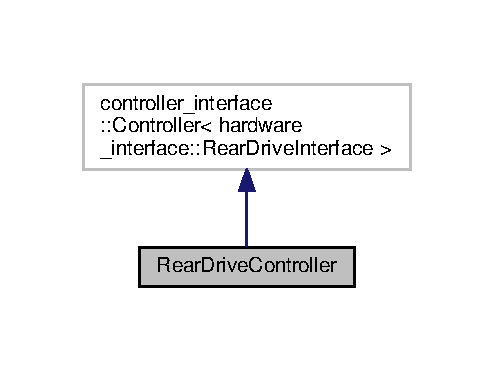
\includegraphics[width=237pt]{classRearDriveController__inherit__graph}
\end{center}
\end{figure}


Collaboration diagram for Rear\+Drive\+Controller\+:\nopagebreak
\begin{figure}[H]
\begin{center}
\leavevmode
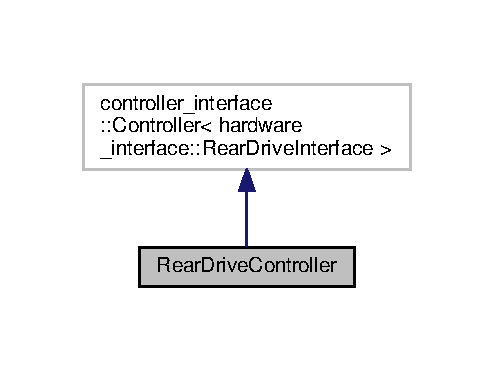
\includegraphics[width=237pt]{classRearDriveController__coll__graph}
\end{center}
\end{figure}
\subsection*{Public Member Functions}
\begin{DoxyCompactItemize}
\item 
bool \hyperlink{classRearDriveController_a024870a0ca82fd44acd0b2b9f2d7e580}{init} (\hyperlink{classhardware__interface_1_1RearDriveInterface}{hardware\+\_\+interface\+::\+Rear\+Drive\+Interface} $\ast$hw, ros\+::\+Node\+Handle \&nh)
\begin{DoxyCompactList}\small\item\em A method to initialize rear drive controller plugin. \end{DoxyCompactList}\item 
void \hyperlink{classRearDriveController_a1990896d6d56922ed2f0d3097a9ea5e4}{update} (const ros\+::\+Time \&time, const ros\+::\+Duration \&period)
\begin{DoxyCompactList}\small\item\em A method to update data sent and received from actual hardware. \end{DoxyCompactList}\item 
void \hyperlink{classRearDriveController_a62dd1436e6ad485642378d7cb65b9960}{starting} (const ros\+::\+Time \&time)
\begin{DoxyCompactList}\small\item\em A method to run while starting rear drive controller. \end{DoxyCompactList}\item 
void \hyperlink{classRearDriveController_a1b3be0cdac62e66726dbe0500008de24}{stopping} (const ros\+::\+Time \&time)
\begin{DoxyCompactList}\small\item\em A method to run for stopping rear drive controller. \end{DoxyCompactList}\end{DoxyCompactItemize}


\subsection{Detailed Description}
A class for basic robot\textquotesingle{}s rear drive controller. 

\subsection{Member Function Documentation}
\mbox{\Hypertarget{classRearDriveController_a024870a0ca82fd44acd0b2b9f2d7e580}\label{classRearDriveController_a024870a0ca82fd44acd0b2b9f2d7e580}} 
\index{Rear\+Drive\+Controller@{Rear\+Drive\+Controller}!init@{init}}
\index{init@{init}!Rear\+Drive\+Controller@{Rear\+Drive\+Controller}}
\subsubsection{\texorpdfstring{init()}{init()}}
{\footnotesize\ttfamily bool Rear\+Drive\+Controller\+::init (\begin{DoxyParamCaption}\item[{\hyperlink{classhardware__interface_1_1RearDriveInterface}{hardware\+\_\+interface\+::\+Rear\+Drive\+Interface} $\ast$}]{hw,  }\item[{ros\+::\+Node\+Handle \&}]{nh }\end{DoxyParamCaption})}



A method to initialize rear drive controller plugin. 


\begin{DoxyParams}{Parameters}
{\em hw} & -\/ Rear drive HW interface instance \\
\hline
{\em nh} & -\/ R\+OS Node\+Handle for communications \\
\hline
\end{DoxyParams}
\begin{DoxyReturn}{Returns}
true 

false 
\end{DoxyReturn}
\mbox{\Hypertarget{classRearDriveController_a62dd1436e6ad485642378d7cb65b9960}\label{classRearDriveController_a62dd1436e6ad485642378d7cb65b9960}} 
\index{Rear\+Drive\+Controller@{Rear\+Drive\+Controller}!starting@{starting}}
\index{starting@{starting}!Rear\+Drive\+Controller@{Rear\+Drive\+Controller}}
\subsubsection{\texorpdfstring{starting()}{starting()}}
{\footnotesize\ttfamily void Rear\+Drive\+Controller\+::starting (\begin{DoxyParamCaption}\item[{const ros\+::\+Time \&}]{time }\end{DoxyParamCaption})\hspace{0.3cm}{\ttfamily [inline]}}



A method to run while starting rear drive controller. 


\begin{DoxyParams}{Parameters}
{\em time} & -\/ Current time or start time \\
\hline
\end{DoxyParams}
\mbox{\Hypertarget{classRearDriveController_a1b3be0cdac62e66726dbe0500008de24}\label{classRearDriveController_a1b3be0cdac62e66726dbe0500008de24}} 
\index{Rear\+Drive\+Controller@{Rear\+Drive\+Controller}!stopping@{stopping}}
\index{stopping@{stopping}!Rear\+Drive\+Controller@{Rear\+Drive\+Controller}}
\subsubsection{\texorpdfstring{stopping()}{stopping()}}
{\footnotesize\ttfamily void Rear\+Drive\+Controller\+::stopping (\begin{DoxyParamCaption}\item[{const ros\+::\+Time \&}]{time }\end{DoxyParamCaption})\hspace{0.3cm}{\ttfamily [inline]}}



A method to run for stopping rear drive controller. 


\begin{DoxyParams}{Parameters}
{\em time} & -\/ Current time or stop time \\
\hline
\end{DoxyParams}
\mbox{\Hypertarget{classRearDriveController_a1990896d6d56922ed2f0d3097a9ea5e4}\label{classRearDriveController_a1990896d6d56922ed2f0d3097a9ea5e4}} 
\index{Rear\+Drive\+Controller@{Rear\+Drive\+Controller}!update@{update}}
\index{update@{update}!Rear\+Drive\+Controller@{Rear\+Drive\+Controller}}
\subsubsection{\texorpdfstring{update()}{update()}}
{\footnotesize\ttfamily void Rear\+Drive\+Controller\+::update (\begin{DoxyParamCaption}\item[{const ros\+::\+Time \&}]{time,  }\item[{const ros\+::\+Duration \&}]{period }\end{DoxyParamCaption})}



A method to update data sent and received from actual hardware. 


\begin{DoxyParams}{Parameters}
{\em time} & -\/ Current time \\
\hline
{\em period} & -\/ Maximum period allowed \\
\hline
\end{DoxyParams}


The documentation for this class was generated from the following files\+:\begin{DoxyCompactItemize}
\item 
controllers/rear\+\_\+drive\+\_\+controller/include/rear\+\_\+drive\+\_\+controller/\hyperlink{rear__drive__controller_8h}{rear\+\_\+drive\+\_\+controller.\+h}\item 
controllers/rear\+\_\+drive\+\_\+controller/src/rear\+\_\+drive\+\_\+controller.\+cpp\end{DoxyCompactItemize}

\hypertarget{classhardware__interface_1_1RearDriveHandle}{}\section{hardware\+\_\+interface\+:\+:Rear\+Drive\+Handle Class Reference}
\label{classhardware__interface_1_1RearDriveHandle}\index{hardware\+\_\+interface\+::\+Rear\+Drive\+Handle@{hardware\+\_\+interface\+::\+Rear\+Drive\+Handle}}


A basic robot\textquotesingle{}s rear drive interface class.  




{\ttfamily \#include $<$rear\+\_\+drive\+\_\+interface.\+h$>$}

\subsection*{Public Member Functions}
\begin{DoxyCompactItemize}
\item 
\mbox{\Hypertarget{classhardware__interface_1_1RearDriveHandle_aadc121a01d6ffc14eb56f372b399a199}\label{classhardware__interface_1_1RearDriveHandle_aadc121a01d6ffc14eb56f372b399a199}} 
\hyperlink{classhardware__interface_1_1RearDriveHandle_aadc121a01d6ffc14eb56f372b399a199}{Rear\+Drive\+Handle} ()=default
\begin{DoxyCompactList}\small\item\em Construct a new default Rear Drive Handle object. \end{DoxyCompactList}\item 
\hyperlink{classhardware__interface_1_1RearDriveHandle_a313af502b28ff7b237b789e44093464c}{Rear\+Drive\+Handle} (const std\+::string \&name, const double $\ast$position, const double $\ast$velocity)
\begin{DoxyCompactList}\small\item\em Construct a new Rear Drive Handle object. \end{DoxyCompactList}\item 
std\+::string \hyperlink{classhardware__interface_1_1RearDriveHandle_a2295641b8ecad58b7064957c64ce28f4}{get\+Name} () const
\begin{DoxyCompactList}\small\item\em Get the name of rear drive handle. \end{DoxyCompactList}\item 
double \hyperlink{classhardware__interface_1_1RearDriveHandle_a214b6bdb767de7f7a4808a03bc95e72a}{get\+Position} () const
\begin{DoxyCompactList}\small\item\em Get the position of rear drive handle. \end{DoxyCompactList}\item 
double \hyperlink{classhardware__interface_1_1RearDriveHandle_ad132a1d990940ed9578824c5084b702b}{get\+Velocity} () const
\begin{DoxyCompactList}\small\item\em Get the velocity of rear drive handle. \end{DoxyCompactList}\item 
const double $\ast$ \hyperlink{classhardware__interface_1_1RearDriveHandle_a003b235bf0a2b64571aa8179d2687664}{get\+Position\+Ptr} () const
\begin{DoxyCompactList}\small\item\em Get the Position Ptr of rear drive handle. \end{DoxyCompactList}\item 
const double $\ast$ \hyperlink{classhardware__interface_1_1RearDriveHandle_a02f8ff9ba88c2642d71ebdafad9122c1}{get\+Velocity\+Ptr} () const
\begin{DoxyCompactList}\small\item\em Get the Velocity Ptr of rear drive handle. \end{DoxyCompactList}\end{DoxyCompactItemize}


\subsection{Detailed Description}
A basic robot\textquotesingle{}s rear drive interface class. 

\subsection{Constructor \& Destructor Documentation}
\mbox{\Hypertarget{classhardware__interface_1_1RearDriveHandle_a313af502b28ff7b237b789e44093464c}\label{classhardware__interface_1_1RearDriveHandle_a313af502b28ff7b237b789e44093464c}} 
\index{hardware\+\_\+interface\+::\+Rear\+Drive\+Handle@{hardware\+\_\+interface\+::\+Rear\+Drive\+Handle}!Rear\+Drive\+Handle@{Rear\+Drive\+Handle}}
\index{Rear\+Drive\+Handle@{Rear\+Drive\+Handle}!hardware\+\_\+interface\+::\+Rear\+Drive\+Handle@{hardware\+\_\+interface\+::\+Rear\+Drive\+Handle}}
\subsubsection{\texorpdfstring{Rear\+Drive\+Handle()}{RearDriveHandle()}}
{\footnotesize\ttfamily hardware\+\_\+interface\+::\+Rear\+Drive\+Handle\+::\+Rear\+Drive\+Handle (\begin{DoxyParamCaption}\item[{const std\+::string \&}]{name,  }\item[{const double $\ast$}]{position,  }\item[{const double $\ast$}]{velocity }\end{DoxyParamCaption})\hspace{0.3cm}{\ttfamily [inline]}}



Construct a new Rear Drive Handle object. 


\begin{DoxyParams}{Parameters}
{\em name} & -\/ Name of rear drive handle \\
\hline
{\em position} & -\/ Position of rear drive handle \\
\hline
{\em velocity} & -\/ Velocity of rear drive handle \\
\hline
\end{DoxyParams}


\subsection{Member Function Documentation}
\mbox{\Hypertarget{classhardware__interface_1_1RearDriveHandle_a2295641b8ecad58b7064957c64ce28f4}\label{classhardware__interface_1_1RearDriveHandle_a2295641b8ecad58b7064957c64ce28f4}} 
\index{hardware\+\_\+interface\+::\+Rear\+Drive\+Handle@{hardware\+\_\+interface\+::\+Rear\+Drive\+Handle}!get\+Name@{get\+Name}}
\index{get\+Name@{get\+Name}!hardware\+\_\+interface\+::\+Rear\+Drive\+Handle@{hardware\+\_\+interface\+::\+Rear\+Drive\+Handle}}
\subsubsection{\texorpdfstring{get\+Name()}{getName()}}
{\footnotesize\ttfamily std\+::string hardware\+\_\+interface\+::\+Rear\+Drive\+Handle\+::get\+Name (\begin{DoxyParamCaption}{ }\end{DoxyParamCaption}) const\hspace{0.3cm}{\ttfamily [inline]}}



Get the name of rear drive handle. 

\begin{DoxyReturn}{Returns}
std\+::string -\/ Name of rear drive handle 
\end{DoxyReturn}
\mbox{\Hypertarget{classhardware__interface_1_1RearDriveHandle_a214b6bdb767de7f7a4808a03bc95e72a}\label{classhardware__interface_1_1RearDriveHandle_a214b6bdb767de7f7a4808a03bc95e72a}} 
\index{hardware\+\_\+interface\+::\+Rear\+Drive\+Handle@{hardware\+\_\+interface\+::\+Rear\+Drive\+Handle}!get\+Position@{get\+Position}}
\index{get\+Position@{get\+Position}!hardware\+\_\+interface\+::\+Rear\+Drive\+Handle@{hardware\+\_\+interface\+::\+Rear\+Drive\+Handle}}
\subsubsection{\texorpdfstring{get\+Position()}{getPosition()}}
{\footnotesize\ttfamily double hardware\+\_\+interface\+::\+Rear\+Drive\+Handle\+::get\+Position (\begin{DoxyParamCaption}{ }\end{DoxyParamCaption}) const\hspace{0.3cm}{\ttfamily [inline]}}



Get the position of rear drive handle. 

\begin{DoxyReturn}{Returns}
double -\/ Position data 
\end{DoxyReturn}
\mbox{\Hypertarget{classhardware__interface_1_1RearDriveHandle_a003b235bf0a2b64571aa8179d2687664}\label{classhardware__interface_1_1RearDriveHandle_a003b235bf0a2b64571aa8179d2687664}} 
\index{hardware\+\_\+interface\+::\+Rear\+Drive\+Handle@{hardware\+\_\+interface\+::\+Rear\+Drive\+Handle}!get\+Position\+Ptr@{get\+Position\+Ptr}}
\index{get\+Position\+Ptr@{get\+Position\+Ptr}!hardware\+\_\+interface\+::\+Rear\+Drive\+Handle@{hardware\+\_\+interface\+::\+Rear\+Drive\+Handle}}
\subsubsection{\texorpdfstring{get\+Position\+Ptr()}{getPositionPtr()}}
{\footnotesize\ttfamily const double$\ast$ hardware\+\_\+interface\+::\+Rear\+Drive\+Handle\+::get\+Position\+Ptr (\begin{DoxyParamCaption}{ }\end{DoxyParamCaption}) const\hspace{0.3cm}{\ttfamily [inline]}}



Get the Position Ptr of rear drive handle. 

\begin{DoxyReturn}{Returns}
const double$\ast$ -\/ Position pointer 
\end{DoxyReturn}
\mbox{\Hypertarget{classhardware__interface_1_1RearDriveHandle_ad132a1d990940ed9578824c5084b702b}\label{classhardware__interface_1_1RearDriveHandle_ad132a1d990940ed9578824c5084b702b}} 
\index{hardware\+\_\+interface\+::\+Rear\+Drive\+Handle@{hardware\+\_\+interface\+::\+Rear\+Drive\+Handle}!get\+Velocity@{get\+Velocity}}
\index{get\+Velocity@{get\+Velocity}!hardware\+\_\+interface\+::\+Rear\+Drive\+Handle@{hardware\+\_\+interface\+::\+Rear\+Drive\+Handle}}
\subsubsection{\texorpdfstring{get\+Velocity()}{getVelocity()}}
{\footnotesize\ttfamily double hardware\+\_\+interface\+::\+Rear\+Drive\+Handle\+::get\+Velocity (\begin{DoxyParamCaption}{ }\end{DoxyParamCaption}) const\hspace{0.3cm}{\ttfamily [inline]}}



Get the velocity of rear drive handle. 

\begin{DoxyReturn}{Returns}
double -\/ Velocity data 
\end{DoxyReturn}
\mbox{\Hypertarget{classhardware__interface_1_1RearDriveHandle_a02f8ff9ba88c2642d71ebdafad9122c1}\label{classhardware__interface_1_1RearDriveHandle_a02f8ff9ba88c2642d71ebdafad9122c1}} 
\index{hardware\+\_\+interface\+::\+Rear\+Drive\+Handle@{hardware\+\_\+interface\+::\+Rear\+Drive\+Handle}!get\+Velocity\+Ptr@{get\+Velocity\+Ptr}}
\index{get\+Velocity\+Ptr@{get\+Velocity\+Ptr}!hardware\+\_\+interface\+::\+Rear\+Drive\+Handle@{hardware\+\_\+interface\+::\+Rear\+Drive\+Handle}}
\subsubsection{\texorpdfstring{get\+Velocity\+Ptr()}{getVelocityPtr()}}
{\footnotesize\ttfamily const double$\ast$ hardware\+\_\+interface\+::\+Rear\+Drive\+Handle\+::get\+Velocity\+Ptr (\begin{DoxyParamCaption}{ }\end{DoxyParamCaption}) const\hspace{0.3cm}{\ttfamily [inline]}}



Get the Velocity Ptr of rear drive handle. 

\begin{DoxyReturn}{Returns}
const double$\ast$ -\/ Velocity pointer 
\end{DoxyReturn}


The documentation for this class was generated from the following file\+:\begin{DoxyCompactItemize}
\item 
hardware\+\_\+interfaces/rear\+\_\+drive\+\_\+interface/include/rear\+\_\+drive\+\_\+interface/\hyperlink{rear__drive__interface_8h}{rear\+\_\+drive\+\_\+interface.\+h}\end{DoxyCompactItemize}

\hypertarget{classhardware__interface_1_1RearDriveInterface}{}\section{hardware\+\_\+interface\+:\+:Rear\+Drive\+Interface Class Reference}
\label{classhardware__interface_1_1RearDriveInterface}\index{hardware\+\_\+interface\+::\+Rear\+Drive\+Interface@{hardware\+\_\+interface\+::\+Rear\+Drive\+Interface}}


A basic robot\textquotesingle{}s rear drive interface class.  




{\ttfamily \#include $<$rear\+\_\+drive\+\_\+interface.\+h$>$}



Inheritance diagram for hardware\+\_\+interface\+:\+:Rear\+Drive\+Interface\+:\nopagebreak
\begin{figure}[H]
\begin{center}
\leavevmode
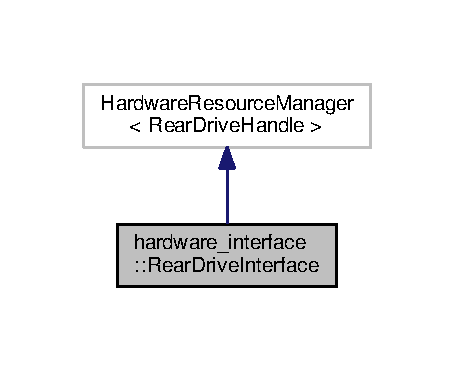
\includegraphics[width=218pt]{classhardware__interface_1_1RearDriveInterface__inherit__graph}
\end{center}
\end{figure}


Collaboration diagram for hardware\+\_\+interface\+:\+:Rear\+Drive\+Interface\+:\nopagebreak
\begin{figure}[H]
\begin{center}
\leavevmode
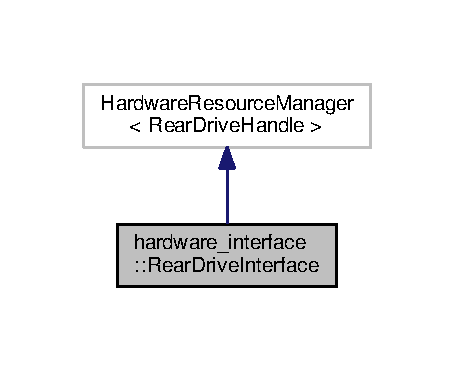
\includegraphics[width=218pt]{classhardware__interface_1_1RearDriveInterface__coll__graph}
\end{center}
\end{figure}


\subsection{Detailed Description}
A basic robot\textquotesingle{}s rear drive interface class. 

The documentation for this class was generated from the following file\+:\begin{DoxyCompactItemize}
\item 
hardware\+\_\+interfaces/rear\+\_\+drive\+\_\+interface/include/rear\+\_\+drive\+\_\+interface/\hyperlink{rear__drive__interface_8h}{rear\+\_\+drive\+\_\+interface.\+h}\end{DoxyCompactItemize}

\hypertarget{classSimulation}{}\section{Simulation Class Reference}
\label{classSimulation}\index{Simulation@{Simulation}}


A basic robot\textquotesingle{}s simulation class.  




{\ttfamily \#include $<$simulation.\+h$>$}

\subsection*{Public Member Functions}
\begin{DoxyCompactItemize}
\item 
\hyperlink{classSimulation_a621e773d9c3168f63d7cb7781f21a344}{Simulation} (ros\+::\+Node\+Handle \&nh)
\begin{DoxyCompactList}\small\item\em A constructor for basic robot\textquotesingle{}s simulation. \end{DoxyCompactList}\item 
\mbox{\Hypertarget{classSimulation_a80fad3f57dfaf195a36f7bc49bc88279}\label{classSimulation_a80fad3f57dfaf195a36f7bc49bc88279}} 
virtual \hyperlink{classSimulation_a80fad3f57dfaf195a36f7bc49bc88279}{$\sim$\+Simulation} ()
\begin{DoxyCompactList}\small\item\em A destructor for basic robot\textquotesingle{}s simulation. \end{DoxyCompactList}\item 
\mbox{\Hypertarget{classSimulation_a418b4eb171471080b9603fa2c0859b02}\label{classSimulation_a418b4eb171471080b9603fa2c0859b02}} 
void \hyperlink{classSimulation_a418b4eb171471080b9603fa2c0859b02}{start\+Sim} ()
\begin{DoxyCompactList}\small\item\em A method to start simulation. \end{DoxyCompactList}\item 
\mbox{\Hypertarget{classSimulation_a3edaab130396016896c2ed49b6051d96}\label{classSimulation_a3edaab130396016896c2ed49b6051d96}} 
void \hyperlink{classSimulation_a3edaab130396016896c2ed49b6051d96}{stop\+Sim} ()
\begin{DoxyCompactList}\small\item\em A method to stop simulation. \end{DoxyCompactList}\item 
int \hyperlink{classSimulation_a22538e804ab0fef459d1af4e1131b091}{get\+Update\+Rate} () const
\begin{DoxyCompactList}\small\item\em A method to get update rate. \end{DoxyCompactList}\end{DoxyCompactItemize}


\subsection{Detailed Description}
A basic robot\textquotesingle{}s simulation class. 

\subsection{Constructor \& Destructor Documentation}
\mbox{\Hypertarget{classSimulation_a621e773d9c3168f63d7cb7781f21a344}\label{classSimulation_a621e773d9c3168f63d7cb7781f21a344}} 
\index{Simulation@{Simulation}!Simulation@{Simulation}}
\index{Simulation@{Simulation}!Simulation@{Simulation}}
\subsubsection{\texorpdfstring{Simulation()}{Simulation()}}
{\footnotesize\ttfamily Simulation\+::\+Simulation (\begin{DoxyParamCaption}\item[{ros\+::\+Node\+Handle \&}]{nh }\end{DoxyParamCaption})}



A constructor for basic robot\textquotesingle{}s simulation. 


\begin{DoxyParams}{Parameters}
{\em nh} & -\/ Nodehandle for R\+OS communication \\
\hline
\end{DoxyParams}


\subsection{Member Function Documentation}
\mbox{\Hypertarget{classSimulation_a22538e804ab0fef459d1af4e1131b091}\label{classSimulation_a22538e804ab0fef459d1af4e1131b091}} 
\index{Simulation@{Simulation}!get\+Update\+Rate@{get\+Update\+Rate}}
\index{get\+Update\+Rate@{get\+Update\+Rate}!Simulation@{Simulation}}
\subsubsection{\texorpdfstring{get\+Update\+Rate()}{getUpdateRate()}}
{\footnotesize\ttfamily int Simulation\+::get\+Update\+Rate (\begin{DoxyParamCaption}{ }\end{DoxyParamCaption}) const}



A method to get update rate. 

\begin{DoxyReturn}{Returns}
int -\/ Update rate 
\end{DoxyReturn}


The documentation for this class was generated from the following files\+:\begin{DoxyCompactItemize}
\item 
simulation/include/simulation/\hyperlink{simulation_8h}{simulation.\+h}\item 
simulation/src/simulation.\+cpp\end{DoxyCompactItemize}

\hypertarget{structState}{}\section{State Struct Reference}
\label{structState}\index{State@{State}}


A struct to represent the robot state.  




{\ttfamily \#include $<$basic\+\_\+robot\+\_\+types.\+h$>$}

\subsection*{Public Member Functions}
\begin{DoxyCompactItemize}
\item 
\hyperlink{structState_afb4608f4a1686ab31d14af3118d702e4}{State} (float p\+\_\+x=0, float p\+\_\+y=0, float p\+\_\+theta=0)
\begin{DoxyCompactList}\small\item\em Construct a new \hyperlink{structState}{State} object. \end{DoxyCompactList}\end{DoxyCompactItemize}
\subsection*{Public Attributes}
\begin{DoxyCompactItemize}
\item 
float \hyperlink{structState_a9948cc668f49246582cfd131b7928f7e}{x}
\item 
float \hyperlink{structState_a89572abb38dea3b1a780ede589a2d59b}{y}
\item 
float \hyperlink{structState_a30afc89f484d7de62a17809c2a70a410}{theta}
\end{DoxyCompactItemize}


\subsection{Detailed Description}
A struct to represent the robot state. 

\subsection{Constructor \& Destructor Documentation}
\mbox{\Hypertarget{structState_afb4608f4a1686ab31d14af3118d702e4}\label{structState_afb4608f4a1686ab31d14af3118d702e4}} 
\index{State@{State}!State@{State}}
\index{State@{State}!State@{State}}
\subsubsection{\texorpdfstring{State()}{State()}}
{\footnotesize\ttfamily State\+::\+State (\begin{DoxyParamCaption}\item[{float}]{p\+\_\+x = {\ttfamily 0},  }\item[{float}]{p\+\_\+y = {\ttfamily 0},  }\item[{float}]{p\+\_\+theta = {\ttfamily 0} }\end{DoxyParamCaption})\hspace{0.3cm}{\ttfamily [inline]}}



Construct a new \hyperlink{structState}{State} object. 


\begin{DoxyParams}{Parameters}
{\em p\+\_\+x} & -\/ X coordinate in space \\
\hline
{\em p\+\_\+y} & -\/ Y coordinate in space \\
\hline
{\em p\+\_\+theta} & -\/ Orientation of robot around Z axis (yaw) \\
\hline
\end{DoxyParams}


\subsection{Member Data Documentation}
\mbox{\Hypertarget{structState_a30afc89f484d7de62a17809c2a70a410}\label{structState_a30afc89f484d7de62a17809c2a70a410}} 
\index{State@{State}!theta@{theta}}
\index{theta@{theta}!State@{State}}
\subsubsection{\texorpdfstring{theta}{theta}}
{\footnotesize\ttfamily float State\+::theta}

Orientation of robot around Z axis (yaw) \mbox{\Hypertarget{structState_a9948cc668f49246582cfd131b7928f7e}\label{structState_a9948cc668f49246582cfd131b7928f7e}} 
\index{State@{State}!x@{x}}
\index{x@{x}!State@{State}}
\subsubsection{\texorpdfstring{x}{x}}
{\footnotesize\ttfamily float State\+::x}

X coordinate in space \mbox{\Hypertarget{structState_a89572abb38dea3b1a780ede589a2d59b}\label{structState_a89572abb38dea3b1a780ede589a2d59b}} 
\index{State@{State}!y@{y}}
\index{y@{y}!State@{State}}
\subsubsection{\texorpdfstring{y}{y}}
{\footnotesize\ttfamily float State\+::y}

Y coordinate in space 

The documentation for this struct was generated from the following file\+:\begin{DoxyCompactItemize}
\item 
basic\+\_\+robot/include/basic\+\_\+robot/\hyperlink{basic__robot__types_8h}{basic\+\_\+robot\+\_\+types.\+h}\end{DoxyCompactItemize}

\chapter{File Documentation}
\hypertarget{basic__robot_8h}{}\section{basic\+\_\+robot/include/basic\+\_\+robot/basic\+\_\+robot.h File Reference}
\label{basic__robot_8h}\index{basic\+\_\+robot/include/basic\+\_\+robot/basic\+\_\+robot.\+h@{basic\+\_\+robot/include/basic\+\_\+robot/basic\+\_\+robot.\+h}}


A file for basic robot\textquotesingle{}s header files.  


{\ttfamily \#include \char`\"{}basic\+\_\+robot/basic\+\_\+robot\+\_\+types.\+h\char`\"{}}\newline
{\ttfamily \#include \char`\"{}system/kinematics.\+h\char`\"{}}\newline
Include dependency graph for basic\+\_\+robot.\+h\+:\nopagebreak
\begin{figure}[H]
\begin{center}
\leavevmode
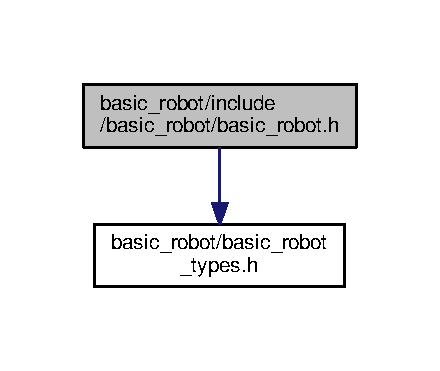
\includegraphics[width=350pt]{basic__robot_8h__incl}
\end{center}
\end{figure}
This graph shows which files directly or indirectly include this file\+:
\nopagebreak
\begin{figure}[H]
\begin{center}
\leavevmode
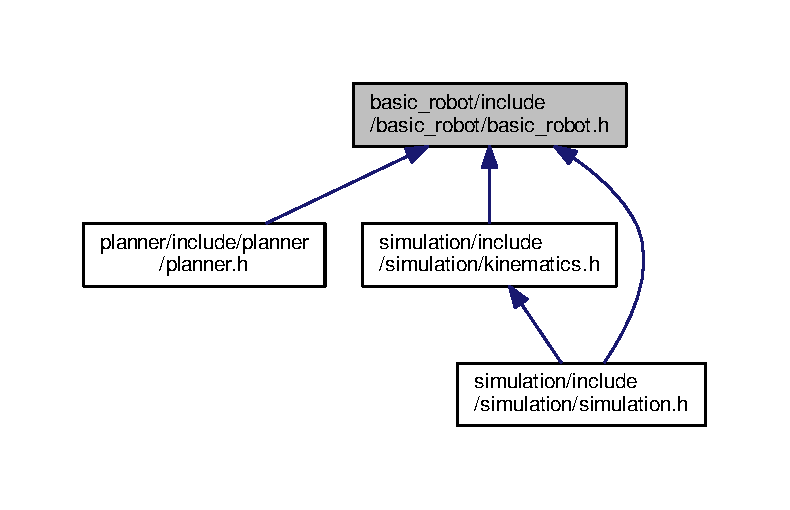
\includegraphics[width=350pt]{basic__robot_8h__dep__incl}
\end{center}
\end{figure}


\subsection{Detailed Description}
A file for basic robot\textquotesingle{}s header files. 

\begin{DoxyAuthor}{Author}
Venkatavaradhan Vembanoor Lakshmi Narayanan (\href{mailto:venkatavaradhan93@gmail.com}{\tt venkatavaradhan93@gmail.\+com}) 
\end{DoxyAuthor}
\begin{DoxyVersion}{Version}
0.\+1 
\end{DoxyVersion}
\begin{DoxyDate}{Date}
2020-\/05-\/10 
\end{DoxyDate}
\begin{DoxyCopyright}{Copyright}
Copyright (c) 2020 
\end{DoxyCopyright}

\hypertarget{basic__robot__types_8h}{}\section{basic\+\_\+robot/include/basic\+\_\+robot/basic\+\_\+robot\+\_\+types.h File Reference}
\label{basic__robot__types_8h}\index{basic\+\_\+robot/include/basic\+\_\+robot/basic\+\_\+robot\+\_\+types.\+h@{basic\+\_\+robot/include/basic\+\_\+robot/basic\+\_\+robot\+\_\+types.\+h}}


A file for basic robot\textquotesingle{}s types.  


This graph shows which files directly or indirectly include this file\+:\nopagebreak
\begin{figure}[H]
\begin{center}
\leavevmode
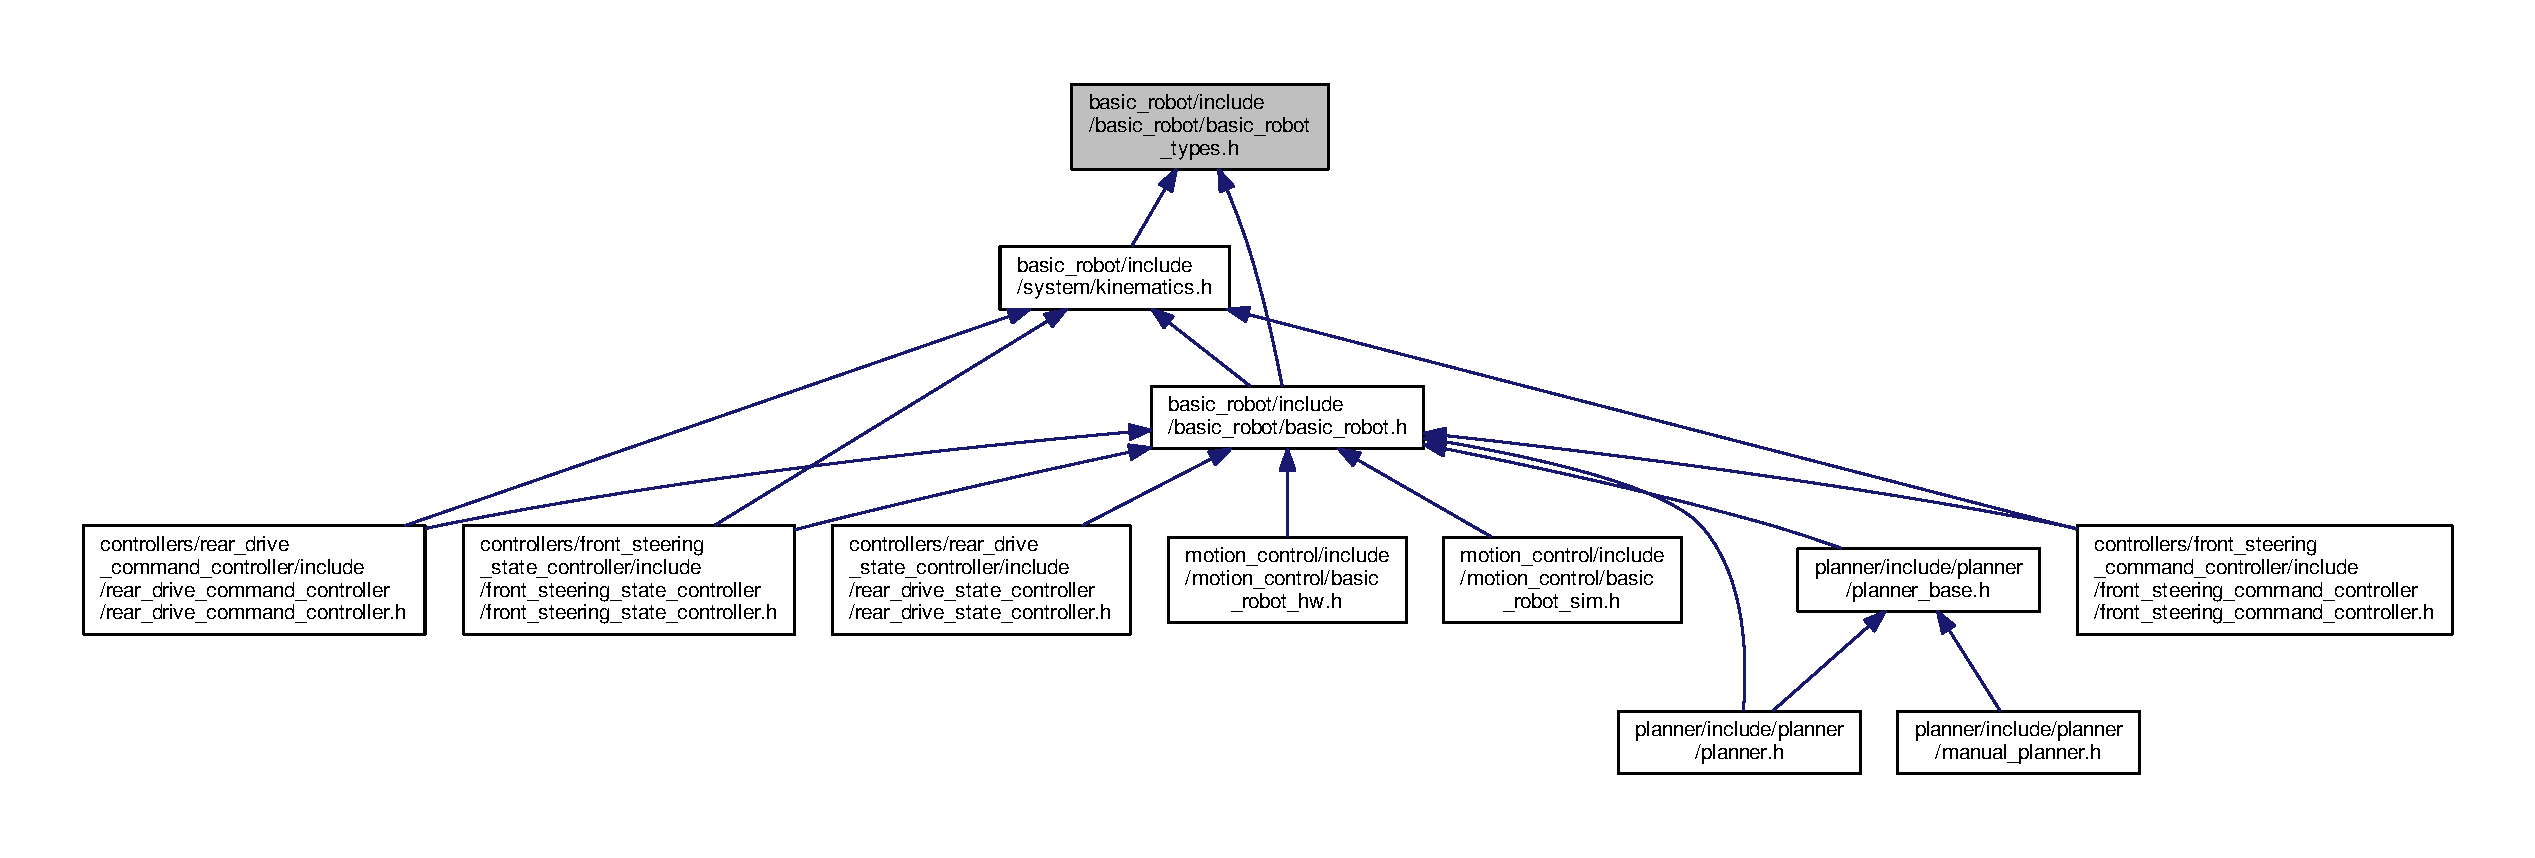
\includegraphics[width=350pt]{basic__robot__types_8h__dep__incl}
\end{center}
\end{figure}
\subsection*{Classes}
\begin{DoxyCompactItemize}
\item 
struct \hyperlink{structState}{State}
\begin{DoxyCompactList}\small\item\em A struct to represent the robot state. \end{DoxyCompactList}\item 
struct \hyperlink{structNoiseParameters}{Noise\+Parameters}
\begin{DoxyCompactList}\small\item\em A struct to represent noise parameters. \end{DoxyCompactList}\item 
struct \hyperlink{structFrontWheel}{Front\+Wheel}
\begin{DoxyCompactList}\small\item\em A struct to represent robot front wheel hub angles. \end{DoxyCompactList}\item 
struct \hyperlink{structRearWheel}{Rear\+Wheel}
\begin{DoxyCompactList}\small\item\em A struct to represent robot rear wheel velocities. \end{DoxyCompactList}\item 
struct \hyperlink{structRobotDimensions}{Robot\+Dimensions}
\begin{DoxyCompactList}\small\item\em A struct to represent basic robot dimensions. \end{DoxyCompactList}\end{DoxyCompactItemize}


\subsection{Detailed Description}
A file for basic robot\textquotesingle{}s types. 

\begin{DoxyAuthor}{Author}
Venkatavaradhan Vembanoor Lakshmi Narayanan (\href{mailto:venkatavaradhan93@gmail.com}{\tt venkatavaradhan93@gmail.\+com}) 
\end{DoxyAuthor}
\begin{DoxyVersion}{Version}
0.\+1 
\end{DoxyVersion}
\begin{DoxyDate}{Date}
2020-\/05-\/10 
\end{DoxyDate}
\begin{DoxyCopyright}{Copyright}
Copyright (c) 2020 
\end{DoxyCopyright}

\hypertarget{rear__drive__controller_8h}{}\section{controllers/rear\+\_\+drive\+\_\+controller/include/rear\+\_\+drive\+\_\+controller/rear\+\_\+drive\+\_\+controller.h File Reference}
\label{rear__drive__controller_8h}\index{controllers/rear\+\_\+drive\+\_\+controller/include/rear\+\_\+drive\+\_\+controller/rear\+\_\+drive\+\_\+controller.\+h@{controllers/rear\+\_\+drive\+\_\+controller/include/rear\+\_\+drive\+\_\+controller/rear\+\_\+drive\+\_\+controller.\+h}}


A basic robot\textquotesingle{}s rear drive controller class.  


{\ttfamily \#include $<$controller\+\_\+interface/controller.\+h$>$}\newline
{\ttfamily \#include $<$pluginlib/class\+\_\+list\+\_\+macros.\+h$>$}\newline
{\ttfamily \#include $<$realtime\+\_\+tools/realtime\+\_\+publisher.\+h$>$}\newline
{\ttfamily \#include $<$ackermann\+\_\+msgs/\+Ackermann\+Drive\+Stamped.\+h$>$}\newline
{\ttfamily \#include \char`\"{}rear\+\_\+drive\+\_\+interface/rear\+\_\+drive\+\_\+interface.\+h\char`\"{}}\newline
Include dependency graph for rear\+\_\+drive\+\_\+controller.\+h\+:
\nopagebreak
\begin{figure}[H]
\begin{center}
\leavevmode
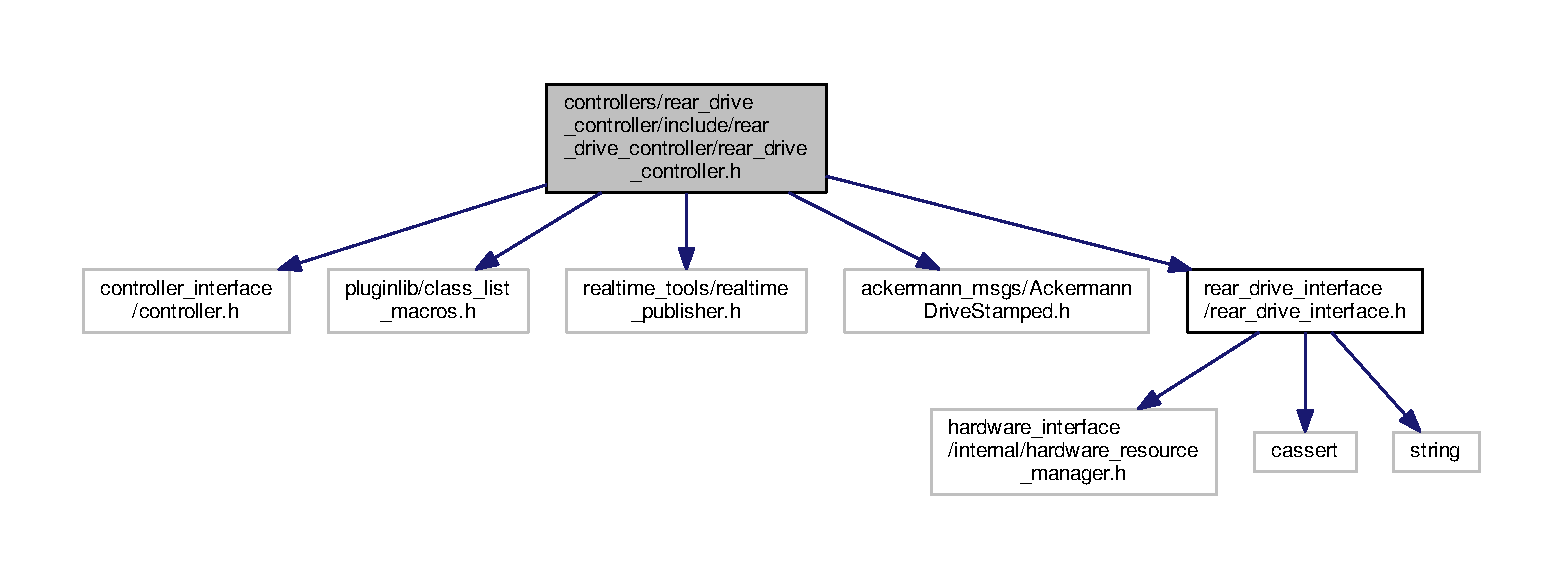
\includegraphics[width=350pt]{rear__drive__controller_8h__incl}
\end{center}
\end{figure}
\subsection*{Classes}
\begin{DoxyCompactItemize}
\item 
class \hyperlink{classRearDriveController}{Rear\+Drive\+Controller}
\begin{DoxyCompactList}\small\item\em A class for basic robot\textquotesingle{}s rear drive controller. \end{DoxyCompactList}\end{DoxyCompactItemize}


\subsection{Detailed Description}
A basic robot\textquotesingle{}s rear drive controller class. 

\begin{DoxyAuthor}{Author}
Venkatavaradhan Vembanoor Lakshmi Narayanan (\href{mailto:venkatavaradhan93@gmail.com}{\tt venkatavaradhan93@gmail.\+com}) 
\end{DoxyAuthor}
\begin{DoxyVersion}{Version}
0.\+1 
\end{DoxyVersion}
\begin{DoxyDate}{Date}
2020-\/05-\/10 
\end{DoxyDate}
\begin{DoxyCopyright}{Copyright}
Copyright (c) 2020 
\end{DoxyCopyright}

\hypertarget{rear__drive__interface_8h}{}\section{hardware\+\_\+interfaces/rear\+\_\+drive\+\_\+interface/include/rear\+\_\+drive\+\_\+interface/rear\+\_\+drive\+\_\+interface.h File Reference}
\label{rear__drive__interface_8h}\index{hardware\+\_\+interfaces/rear\+\_\+drive\+\_\+interface/include/rear\+\_\+drive\+\_\+interface/rear\+\_\+drive\+\_\+interface.\+h@{hardware\+\_\+interfaces/rear\+\_\+drive\+\_\+interface/include/rear\+\_\+drive\+\_\+interface/rear\+\_\+drive\+\_\+interface.\+h}}


A basic robot\textquotesingle{}s rear drive hw interface class.  


{\ttfamily \#include $<$hardware\+\_\+interface/internal/hardware\+\_\+resource\+\_\+manager.\+h$>$}\newline
{\ttfamily \#include $<$cassert$>$}\newline
{\ttfamily \#include $<$string$>$}\newline
Include dependency graph for rear\+\_\+drive\+\_\+interface.\+h\+:\nopagebreak
\begin{figure}[H]
\begin{center}
\leavevmode
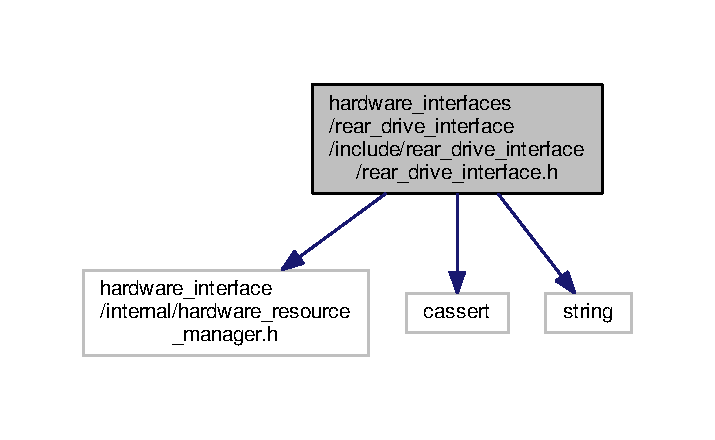
\includegraphics[width=343pt]{rear__drive__interface_8h__incl}
\end{center}
\end{figure}
This graph shows which files directly or indirectly include this file\+:
\nopagebreak
\begin{figure}[H]
\begin{center}
\leavevmode
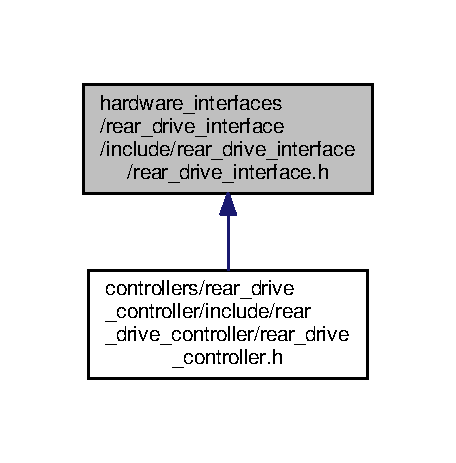
\includegraphics[width=219pt]{rear__drive__interface_8h__dep__incl}
\end{center}
\end{figure}
\subsection*{Classes}
\begin{DoxyCompactItemize}
\item 
class \hyperlink{classhardware__interface_1_1RearDriveHandle}{hardware\+\_\+interface\+::\+Rear\+Drive\+Handle}
\begin{DoxyCompactList}\small\item\em A basic robot\textquotesingle{}s rear drive interface class. \end{DoxyCompactList}\item 
class \hyperlink{classhardware__interface_1_1RearDriveInterface}{hardware\+\_\+interface\+::\+Rear\+Drive\+Interface}
\begin{DoxyCompactList}\small\item\em A basic robot\textquotesingle{}s rear drive interface class. \end{DoxyCompactList}\end{DoxyCompactItemize}


\subsection{Detailed Description}
A basic robot\textquotesingle{}s rear drive hw interface class. 

\begin{DoxyAuthor}{Author}
Venkatavaradhan Vembanoor Lakshmi Narayanan (\href{mailto:venkatavaradhan93@gmail.com}{\tt venkatavaradhan93@gmail.\+com}) 
\end{DoxyAuthor}
\begin{DoxyVersion}{Version}
0.\+1 
\end{DoxyVersion}
\begin{DoxyDate}{Date}
2020-\/05-\/10 
\end{DoxyDate}
\begin{DoxyCopyright}{Copyright}
Copyright (c) 2020 
\end{DoxyCopyright}

\hypertarget{planner_8h}{}\section{planner/include/planner/planner.h File Reference}
\label{planner_8h}\index{planner/include/planner/planner.\+h@{planner/include/planner/planner.\+h}}


A class for basic robot\textquotesingle{}s navigation.  


{\ttfamily \#include $<$ros/ros.\+h$>$}\newline
{\ttfamily \#include $<$pluginlib/class\+\_\+loader.\+h$>$}\newline
{\ttfamily \#include $<$ackermann\+\_\+msgs/\+Ackermann\+Drive\+Stamped.\+h$>$}\newline
{\ttfamily \#include \char`\"{}basic\+\_\+robot/basic\+\_\+robot.\+h\char`\"{}}\newline
{\ttfamily \#include \char`\"{}basic\+\_\+robot/\+Mode.\+h\char`\"{}}\newline
{\ttfamily \#include \char`\"{}basic\+\_\+robot/\+Set\+Mode.\+h\char`\"{}}\newline
{\ttfamily \#include \char`\"{}planner/planner\+\_\+base.\+h\char`\"{}}\newline
Include dependency graph for planner.\+h\+:\nopagebreak
\begin{figure}[H]
\begin{center}
\leavevmode
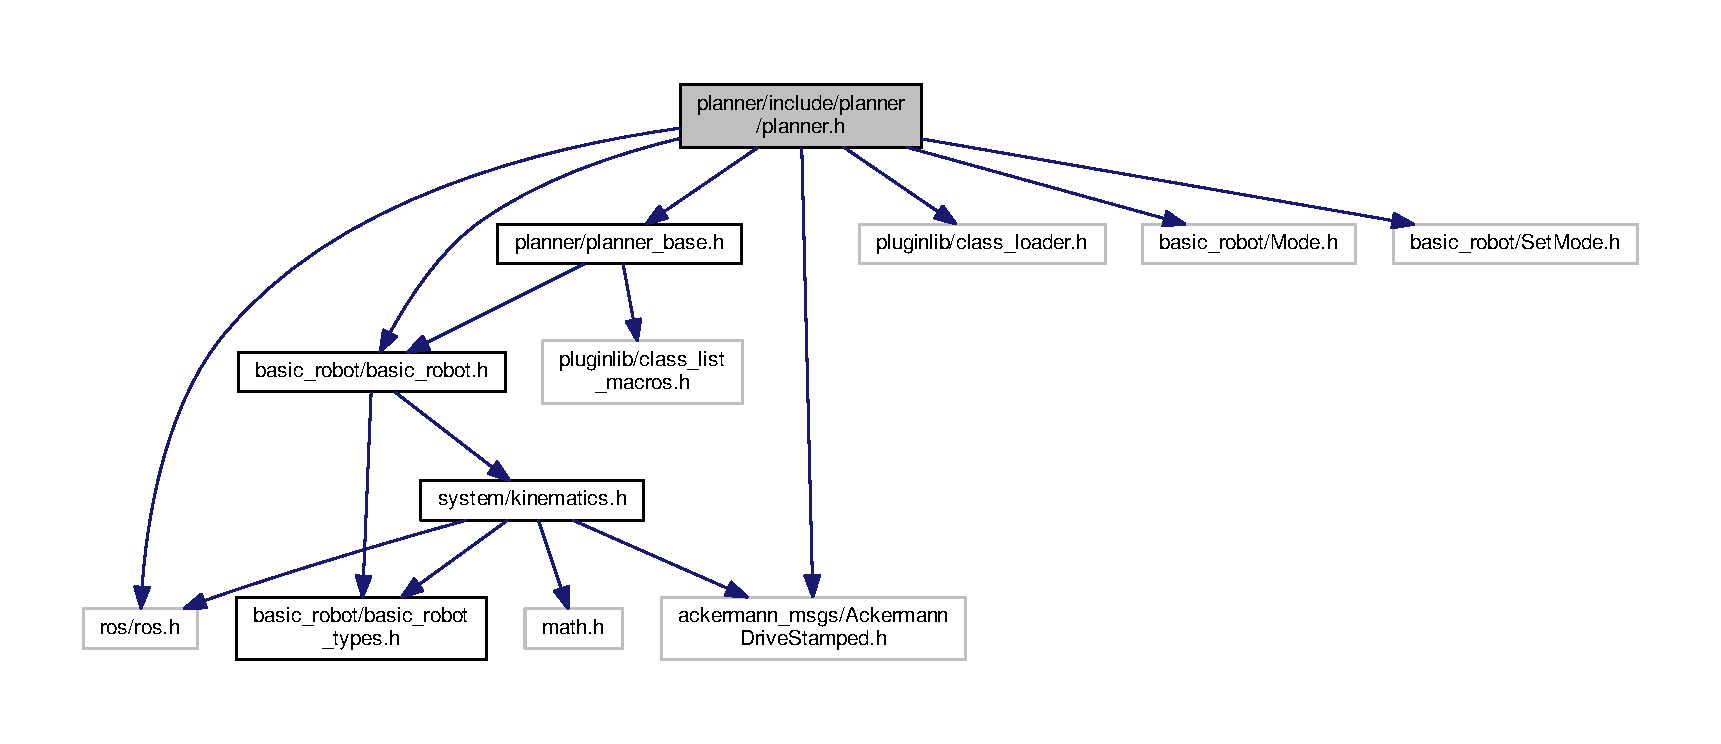
\includegraphics[width=350pt]{planner_8h__incl}
\end{center}
\end{figure}
\subsection*{Classes}
\begin{DoxyCompactItemize}
\item 
class \hyperlink{classPlanner}{Planner}
\begin{DoxyCompactList}\small\item\em A basic robot\textquotesingle{}s planner class. \end{DoxyCompactList}\end{DoxyCompactItemize}


\subsection{Detailed Description}
A class for basic robot\textquotesingle{}s navigation. 

\begin{DoxyAuthor}{Author}
Venkatavaradhan Vembanoor Lakshmi Narayanan (\href{mailto:venkatavaradhan93@gmail.com}{\tt venkatavaradhan93@gmail.\+com}) 
\end{DoxyAuthor}
\begin{DoxyVersion}{Version}
0.\+1 
\end{DoxyVersion}
\begin{DoxyDate}{Date}
2020-\/03-\/31 
\end{DoxyDate}
\begin{DoxyCopyright}{Copyright}
Copyright (c) 2020 
\end{DoxyCopyright}

\hypertarget{kinematics_8h}{}\section{basic\+\_\+robot/include/system/kinematics.h File Reference}
\label{kinematics_8h}\index{basic\+\_\+robot/include/system/kinematics.\+h@{basic\+\_\+robot/include/system/kinematics.\+h}}


A class for basic robot\textquotesingle{}s kinematics.  


{\ttfamily \#include $<$ros/ros.\+h$>$}\newline
{\ttfamily \#include $<$ackermann\+\_\+msgs/\+Ackermann\+Drive\+Stamped.\+h$>$}\newline
{\ttfamily \#include $<$math.\+h$>$}\newline
{\ttfamily \#include \char`\"{}basic\+\_\+robot/basic\+\_\+robot\+\_\+types.\+h\char`\"{}}\newline
Include dependency graph for kinematics.\+h\+:\nopagebreak
\begin{figure}[H]
\begin{center}
\leavevmode
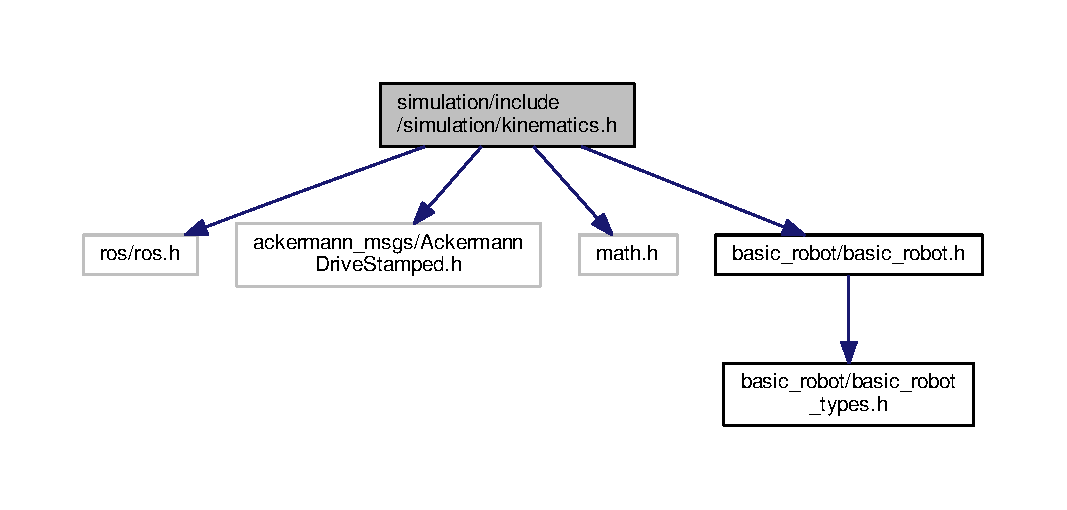
\includegraphics[width=350pt]{kinematics_8h__incl}
\end{center}
\end{figure}
This graph shows which files directly or indirectly include this file\+:\nopagebreak
\begin{figure}[H]
\begin{center}
\leavevmode
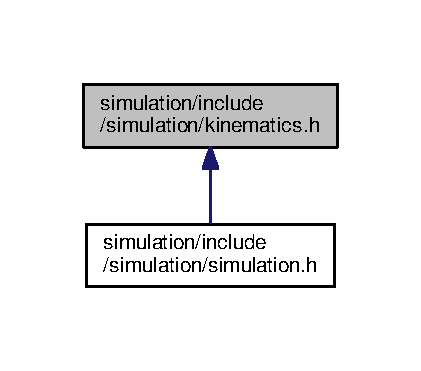
\includegraphics[width=350pt]{kinematics_8h__dep__incl}
\end{center}
\end{figure}
\subsection*{Classes}
\begin{DoxyCompactItemize}
\item 
class \hyperlink{classKinematics}{Kinematics}
\begin{DoxyCompactList}\small\item\em A basic robot\textquotesingle{}s kinematics class. \end{DoxyCompactList}\end{DoxyCompactItemize}


\subsection{Detailed Description}
A class for basic robot\textquotesingle{}s kinematics. 

\begin{DoxyAuthor}{Author}
Venkatavaradhan Vembanoor Lakshmi Narayanan (\href{mailto:venkatavaradhan93@gmail.com}{\tt venkatavaradhan93@gmail.\+com}) 
\end{DoxyAuthor}
\begin{DoxyVersion}{Version}
0.\+1 
\end{DoxyVersion}
\begin{DoxyDate}{Date}
2020-\/03-\/28 
\end{DoxyDate}
\begin{DoxyCopyright}{Copyright}
Copyright (c) 2020 
\end{DoxyCopyright}

\hypertarget{map_8h}{}\section{simulation/include/simulation/map.h File Reference}
\label{map_8h}\index{simulation/include/simulation/map.\+h@{simulation/include/simulation/map.\+h}}


A class to load map from map server.  


{\ttfamily \#include $<$ros/ros.\+h$>$}\newline
{\ttfamily \#include $<$nav\+\_\+msgs/\+Occupancy\+Grid.\+h$>$}\newline
Include dependency graph for map.\+h\+:\nopagebreak
\begin{figure}[H]
\begin{center}
\leavevmode
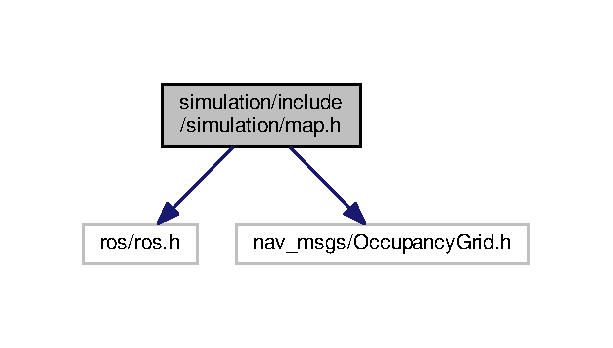
\includegraphics[width=294pt]{map_8h__incl}
\end{center}
\end{figure}
\subsection*{Classes}
\begin{DoxyCompactItemize}
\item 
class \hyperlink{classMap}{Map}
\begin{DoxyCompactList}\small\item\em A basic robot\textquotesingle{}s map class. \end{DoxyCompactList}\end{DoxyCompactItemize}


\subsection{Detailed Description}
A class to load map from map server. 

\begin{DoxyAuthor}{Author}
Venkatavaradhan Vembanoor Lakshmi Narayanan (\href{mailto:venkatavaradhan93@gmail.com}{\tt venkatavaradhan93@gmail.\+com}) 
\end{DoxyAuthor}
\begin{DoxyVersion}{Version}
0.\+1 
\end{DoxyVersion}
\begin{DoxyDate}{Date}
2020-\/03-\/28 
\end{DoxyDate}
\begin{DoxyCopyright}{Copyright}
Copyright (c) 2020 
\end{DoxyCopyright}

\hypertarget{simulation_8h}{}\section{simulation/include/simulation/simulation.h File Reference}
\label{simulation_8h}\index{simulation/include/simulation/simulation.\+h@{simulation/include/simulation/simulation.\+h}}


A class for basic robot\textquotesingle{}s simulation.  


{\ttfamily \#include $<$ros/ros.\+h$>$}\newline
{\ttfamily \#include $<$tf2/\+Linear\+Math/\+Quaternion.\+h$>$}\newline
{\ttfamily \#include $<$tf2\+\_\+ros/transform\+\_\+broadcaster.\+h$>$}\newline
{\ttfamily \#include $<$geometry\+\_\+msgs/\+Transform\+Stamped.\+h$>$}\newline
{\ttfamily \#include $<$ackermann\+\_\+msgs/\+Ackermann\+Drive\+Stamped.\+h$>$}\newline
{\ttfamily \#include $<$boost/thread.\+hpp$>$}\newline
{\ttfamily \#include $<$random$>$}\newline
{\ttfamily \#include \char`\"{}basic\+\_\+robot/basic\+\_\+robot.\+h\char`\"{}}\newline
Include dependency graph for simulation.\+h\+:\nopagebreak
\begin{figure}[H]
\begin{center}
\leavevmode
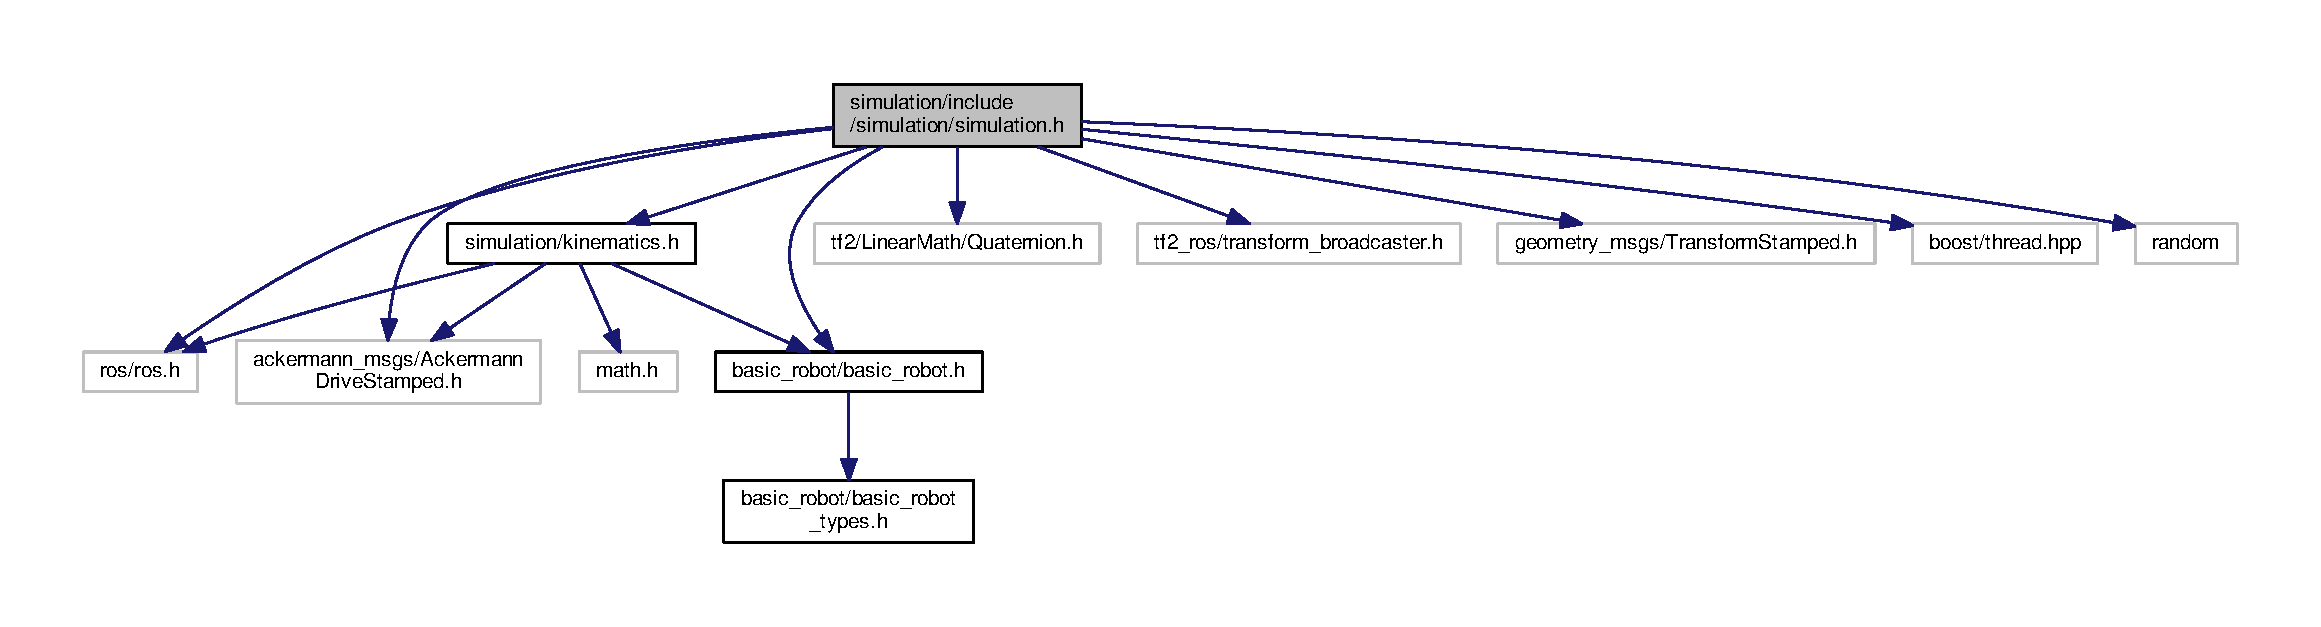
\includegraphics[width=350pt]{simulation_8h__incl}
\end{center}
\end{figure}
\subsection*{Classes}
\begin{DoxyCompactItemize}
\item 
class \hyperlink{classSimulation}{Simulation}
\begin{DoxyCompactList}\small\item\em A basic robot\textquotesingle{}s simulation class. \end{DoxyCompactList}\end{DoxyCompactItemize}


\subsection{Detailed Description}
A class for basic robot\textquotesingle{}s simulation. 

\begin{DoxyAuthor}{Author}
Venkatavaradhan Vembanoor Lakshmi Narayanan (\href{mailto:venkatavaradhan93@gmail.com}{\tt venkatavaradhan93@gmail.\+com}) 
\end{DoxyAuthor}
\begin{DoxyVersion}{Version}
0.\+1 
\end{DoxyVersion}
\begin{DoxyDate}{Date}
2020-\/03-\/29 
\end{DoxyDate}
\begin{DoxyCopyright}{Copyright}
Copyright (c) 2020 
\end{DoxyCopyright}

%--- End generated contents ---

% Index
\backmatter
\newpage
\phantomsection
\clearemptydoublepage
\addcontentsline{toc}{chapter}{Index}
\printindex

\end{document}
